% ===== 原文 pp.90–105（PDF pp.97–112） =====
% [原文 p.90]
\chapter{三角范畴}

本章在叙述三角范畴的定义与基本性质之后，作为其典型例，讨论加法范畴 $\cC$ 的同伦范畴 $K(\cC)$ 所构成的三角范畴，并进一步确认阿贝尔范畴 $\cC$ 的导出范畴 $D(\cC)$ 构成三角范畴。5.5 节讨论三角范畴的 DG 增广。同伦范畴、导出范畴等我们通常处理的三角范畴都自然地具有 DG 增广。对于具有 DG 增广的三角范畴，若干更强的性质成立。5.6 节、5.7 节讨论三角范畴中的附加结构。这些讨论包含艰深的内容，但这些结构将在第 6 章中得到应用。

\section{三角范畴}

首先叙述三角范畴的定义，然后讨论该定义的含义。

\subsection{三角范畴与三角函子}

三角范畴定义为具有正合三角结构的加法范畴。

% [Tutor Note: 本节术语首现：三角范畴（triangulated category）、三角序列（triangle）、正合三角序列（exact triangle）、平移函子（shift functor / translation functor）、八面体公理（octahedral axiom）。底本把「完全三角系列」用作英文 exact triangle 的译名，本译本按 glossary 统一作「正合三角序列」；书中「完全」一律对应 exact。]

\begin{definition}{5.1}
设 $\cT$ 为带有加法自同构函子 $T\colon\cT\to\cT$ 的加法范畴。即，$T$ 是从 $\cT$ 到 $\cT$ 自身的加性同构函子（定义 4.13）。对对象 $X,Y,Z\in\cT$ 与态射 $u\colon X\to Y$，$v\colon Y\to Z$，$w\colon Z\to T(X)$ 的组
\[
(X,Y,Z;u,v,w) := X \xrightarrow{\,u\,} Y \xrightarrow{\,v\,} Z \xrightarrow{\,w\,} T(X)
\]
称为 $\cT$ 中的三角序列（triangle）。
\end{definition}

\begin{remark}{5.2}
正如名称所示，三角序列 $(X,Y,Z;u,v,w)$ 也常表示为
\[
\begin{tikzcd}[row sep=2.2em, column sep=3.4em]
X \arrow[rr,"u"] & & Y \arrow[dl,"v"] \\
{} & Z \arrow[ur,"w\,(+1)"'] &
\end{tikzcd}
,\qquad
\begin{tikzcd}[row sep=2.2em, column sep=3.4em]
X \arrow[rr,"u"] & & Y \arrow[dl,"v"] \\
{} & Z \arrow[ur,dashed,"w"'] &
\end{tikzcd}
\]
等形式。（注意 $w\colon Z\to T(X)$ 的写法。）
\end{remark}

% [Tutor Note: 原文 p.90 注意 5.2 的两个三角形：左侧实线箭头旁标「$w\,(+1)$」，右侧虚线箭头旁标「$w$」。两者是同一三角序列 $X\xrightarrow{u}Y\xrightarrow{v}Z\xrightarrow{w}T(X)$ 的两种画法，$(+1)$ 表示该箭头是次数 $+1$ 的态射（即落点为 $T(X)$ 而非 $X$）；以虚线画箭头是「该箭头经过平移」的另一惯例。可验证锚点：取 $\cT=K(\mathbf{Ab})$、$X=Y=Z=0$ 时三角序列退化为 $0\to 0\to 0\to 0$；取 $u=\id_X$、$Z=0$，则 (Tr1) 给出正合三角序列 $X\xrightarrow{\id_X}X\to 0\to T(X)$。]

% [原文 p.91]
\begin{definition}{5.3}
设 $\cT$ 为带有加法自同构函子 $T\colon\cT\to\cT$ 的加法范畴。对 $\cT$ 的三角序列 $(X,Y,Z;u,v,w)$，$(X',Y',Z';u',v',w')$，若存在态射 $f\colon X\to X'$，$g\colon Y\to Y'$，$h\colon Z\to Z'$ 使图表
\[
\begin{tikzcd}[row sep=2.2em, column sep=2.6em]
X \arrow[r,"u"] \arrow[d,"f"] & Y \arrow[r,"v"] \arrow[d,"g"] & Z \arrow[r,"w"] \arrow[d,"h"] & T(X) \arrow[d,"T(f)"] \\
X' \arrow[r,"u'"] & Y' \arrow[r,"v'"] & Z' \arrow[r,"w'"] & T(X')
\end{tikzcd}
\]
交换，则称 $(f,g,h)\colon(X,Y,Z;u,v,w)\to(X',Y',Z';u',v',w')$ 为三角序列的态射（morphism of triangles）。特别地，当 $f,g,h$ 全为同构态射时，三角序列的态射 $(f,g,h)$ 称为同构态射（isomorphism），并称 $(X,Y,Z;u,v,w)$ 与 $(X',Y',Z';u',v',w')$ 同构（isomorphic）。
\end{definition}

\begin{definition}{5.4}
设 $\cT$ 为带有加法自同构函子 $T\colon\cT\to\cT$ 的加法范畴。以下 (Tr0)–(Tr5) 称为正合三角序列的公理（axiom of exact triangles）。
\begin{enumerate}[start=0, label=(Tr\arabic*), leftmargin=4.6em, itemsep=0.35em]
\item 与某个正合三角序列（作为三角序列）同构的三角序列都是正合三角序列。
\item 三角序列 $X \xrightarrow{\id_X} X \to 0 \to T(X)$ 是正合三角序列。
\item 对任意态射 $f\colon X\to Y$，存在某个正合三角序列
\[
(X,Y,Z;f,v,w) := X \xrightarrow{\,f\,} Y \xrightarrow{\,v\,} Z \xrightarrow{\,w\,} T(X).
\]
\item 三角序列 $X \xrightarrow{u} Y \xrightarrow{v} Z \xrightarrow{w} T(X)$ 正合，当且仅当三角序列 $Y \xrightarrow{v} Z \xrightarrow{w} T(X) \xrightarrow{T(u)} T(Y)$ 也正合。
\item 对任意交换图表
\[
\begin{tikzcd}[row sep=2.2em, column sep=3.6em]
X \arrow[r,"u"] \arrow[d,"f"] & Y \arrow[d,"g"] \\
X' \arrow[r,"u'"] & Y'
\end{tikzcd}
\]
与两个正合三角序列 $(X,Y,Z;u,v,w)$，$(X',Y',Z';u',v',w')$，存在它们之间（作为三角序列的）态射
\[
\begin{tikzcd}[row sep=2.2em, column sep=2.6em]
X \arrow[r,"u"] \arrow[d,"f"] & Y \arrow[r,"v"] \arrow[d,"g"] & Z \arrow[r,"w"] \arrow[d,"h"] & T(X) \arrow[d,"T(f)"] \\
X' \arrow[r,"u'"] & Y' \arrow[r,"v'"] & Z' \arrow[r,"w'"] & T(X')
\end{tikzcd}
\]
（但 $h$ 未必唯一）。
% [原文 p.92]
\item 对态射 $u\colon X\to Y$，$v\colon Y\to Z$ 及其合成 $v\circ u\colon X\to Z$，考虑对应的正合三角序列
\[
X \xrightarrow{u} Y \to Z' \to T(X),\qquad
Y \xrightarrow{v} Z \to X' \to T(Y),\qquad
X \xrightarrow{v\circ u} Z \to Y' \to T(X).
\]
此时，存在正合三角序列 $Z'\to Y'\to X'\to T(Z')$，并且存在包含这四个正合三角序列的如下交换图表。
\[
\begin{tikzcd}[row sep=2.4em, column sep=2.5em]
{} & T^{-1}(X') \arrow[r,equal] \arrow[d,"u'"'] & T^{-1}(X') \arrow[d] & {} \\
X \arrow[r,"u"] \arrow[d,equal,"\id_X"'] & Y \arrow[r] \arrow[d,"v"'] & Z' \arrow[r] \arrow[d] & TX \arrow[d,equal,"\id_{TX}"'] \\
X \arrow[r] & Z \arrow[r] \arrow[d] & Y' \arrow[r] \arrow[d] & TX \arrow[d,"T(u)"] \\
{} & X' \arrow[r,equal] & X' \arrow[r,"T(u')"'] & TY
\end{tikzcd}
\]
\end{enumerate}
\end{definition}

% [Tutor Note: 底本 p.92 的 (Tr5) 图形是作者 2014 年正誤表（八面体公理专项，PDF pp.222–223 = E08/E09）订正的对象。底本图 (1) 缺少右下角的交换方块，即缺少 $TX\xrightarrow{T(u)}TY$ 与 $X'\xrightarrow{T(u')}TY$ 两条边（原图 (1) 中 $Y'\to TX$ 与 $Y'\to X'$ 已有）；本译本已按订正后图 (2) 补全该方块。正誤表同时把 (Tr5) 的叙述改为「存在完全三角系列 $Z'\to Y'\to X'\to T^{-1}$」，据图 (2) 该系列实为 $T^{-1}(X')\to Z'\to Y'\to X'$，也就是 $Z'\to Y'\to X'\to T(Z')$ 的旋转；底本文字此处印作「$T^{-1}$」应视为省略了自变量。批注依据：正誤表 2014-05-24 版「p.92 に関する订正」。]

\begin{remark}{5.5}
公理 (Tr5) 就是所谓的八面体公理（octahedral axiom）。事实上，写出如下八面体图表往往更便于把握。
\[
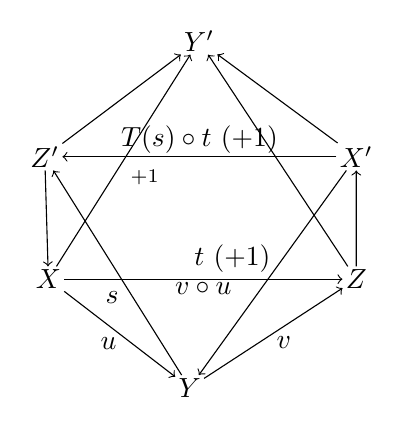
\begin{tikzpicture}[scale=0.92, every node/.style={inner sep=1pt}]
\node (Yp) at (0,2.66) {$Y'$};
\node (Zp) at (-2.13,1.06) {$Z'$};
\node (Xp) at (2.17,1.06) {$X'$};
\node (X)  at (-2.08,-0.63) {$X$};
\node (Z)  at (2.17,-0.63) {$Z$};
\node (Y)  at (-0.13,-2.13) {$Y$};
\draw[->] (Zp) -- (Yp);
\draw[->] (X)  -- (Yp);
\draw[->] (Xp) -- (Yp);
\draw[->] (Z)  -- (Yp);
\draw[->] (Xp) -- node[above] {$T(s)\circ t\ (+1)$} (Zp);
\draw[->] (Zp) -- (X);
\draw[->] (Z)  -- (Xp);
\draw[->] (X)  -- node[below] {$v\circ u$} (Z);
\draw[->] (X)  -- node[below left] {$u$} (Y);
\draw[->] (Y)  -- node[below right] {$v$} (Z);
\draw[->] (Y)  -- (Zp);
\draw[->] (Xp) -- (Y);
\node at (-1.20,-0.88) {$s$};
\node at (0.46,-0.34) {$t\ (+1)$};
\node at (-0.75,0.78) {$\scriptstyle +1$};
\end{tikzpicture}
\]
\end{remark}

% [Tutor Note: 八面体的 6 个顶点中，$Z'$、$X'$、$Y'$ 分别是 $u$、$v$、$v\circ u$ 的写像锥；8 个三角面里恰有 4 个确定正合三角序列（$X\to Y\to Z'$、$Y\to Z\to X'$、$X\to Z\to Y'$、$Z'\to Y'\to X'$），另 4 个面只表示态射的合成。这可作为检查图是否画全的锚点：12 条棱正好分成 4 个三角形（每个 3 条）与 4 个合成四边形。据正誤表 E09，八面体中被「一分为二」的三个四边形里，有一个因箭头方向而不能成为交换图表，其余两个正对应 (5.3) 与 (5.4) 讨论中所用的图 (5) 与图 (3)。图中 $s,t$ 是作者对所取态射的命名，$(+1)$ 表示相应箭头是次数 $+1$ 的态射。]

\begin{definition}{5.6}[三角范畴]
设 $\cT$ 为带有加法自同构函子 $T\colon\cT\to\cT$ 的加法范畴。当 $\cT$ 具有满足正合三角序列公理的正合三角序列类时，称 $\cT$ 具有正合三角结构（exact triangle），此时 $\cT$ 称为三角范畴（triangulated category）。在三角范畴 $\cT$ 中，其加法自同构函子 $T\colon\cT\to\cT$ 称为平移函子（shift functor, translation functor）。当三角范畴 $\cT$ 是域 $K$ 上的加法范畴时，称 $\cT$ 为 $K$ 上的三角范畴。
\end{definition}

关于由公理 (Tr0)–(Tr5) 导出的正合三角序列的性质，将在下节讨论。

% [Tutor Note: 此处底本原文作「次章で議論する」，但紧接的 5.1.2 小节（「完全三角系列から従う事実について」）即在本书范围内讨论此事，故按内容译作「下节」。]

\begin{definition}{5.7}
对三角范畴 $\cT,\cT'$，分别以 $T,T'$ 记 $\cT,\cT'$ 的平移函子。加法函子 $F\colon\cT\to\cT'$ 当
\begin{itemize}[leftmargin=2em, itemsep=0.2em]
\item $F\circ T = T'\circ F$，
% [原文 p.93]
\item 对 $\cT$ 的任意正合三角序列 $(X,Y,Z;u,v,w)$，$(F(X),F(Y),F(Z);F(u),F(v),F(w))$ 都是 $\cT'$ 的正合三角序列
\end{itemize}
时，称为三角函子（triangle functor）。
\end{definition}

\begin{definition}{5.8}
三角范畴 $\cT,\cT'$ 之间的三角函子 $F\colon\cT\to\cT'$，当它也是范畴等价函子时，称为三角范畴等价函子。当存在从 $\cT$ 到 $\cT'$ 的三角范畴等价函子时，称 $\cT$ 与 $\cT'$ 三角范畴等价（triangulated equivalent）。
\end{definition}

\subsection{由正合三角序列导出的事实}

讨论由前节的正合三角序列公理（定义 5.4）导出的性质。

\begin{lemma}{5.9}
设 $\cT$ 为三角范畴。对 $\cT$ 的正合三角序列
\[
(X,Y,Z;u,v,w) = X \xrightarrow{\,u\,} Y \xrightarrow{\,v\,} Z \xrightarrow{\,w\,} T(X),
\]
有 $v\circ u = 0$，$w\circ v = 0$，$T(u)\circ w = 0$。
\end{lemma}

\begin{proof}
由 (Tr1) 存在正合三角序列 $(X,X,0;\id_X,0,0)$，且由 (Tr4) 存在正合三角序列之间的态射 $(X,X,0;\id_X,0,0)\to(X,Y,Z;u,v,w)$。
\[
\begin{tikzcd}[row sep=2.2em, column sep=2.6em]
X \arrow[r,"\id_X"] \arrow[d,"\id_X"] & X \arrow[r,"0"] \arrow[d,"u"] & 0 \arrow[r,"0"] \arrow[d,"0"] & T(X) \arrow[d,"\id_{T(X)}"] \\
X \arrow[r,"u"] & Y \arrow[r,"v"] & Z \arrow[r,"w"] & T(X)
\end{tikzcd}
\]
这里，由上行的正合三角序列的第 2 个 $X$ 到下行的正合三角序列的 $Z$ 的合成态射们的交换性，得到 $v\circ u = 0$。同样地可得到 $w\circ v = 0$，$T(u)\circ w = 0$ 等，而这一事实也可由 (Tr3) 导出。
\end{proof}

% [Tutor Note: 底本 p.93 此处印作「(Tr2) より完全三角系列の間の射 $(X,Y,Z;u,v,w)\to(X,X,0;\id_X,0,0)$ が存在する」。据作者正誤表（2014-05-20 版）p.93 条（带 ♠ 的更新项），应订正为「(Tr4) より完全三角系列の間の射 $(X,X,0;\id_X,0,0)\to(X,Y,Z;u,v,w)$ が存在する」：即所用公理是 (Tr4)（并非 (Tr2)），方向也是自平凡三角序列指向给定三角序列。本译本正文按订正后内容翻译，图本身（上行 $(X,X,0)$、下行 $(X,Y,Z)$）底本无误。]
% [Tutor Note: 结论里三个等式的来历可作可验证锚点：$v\circ u=0$ 由上方方块 $(X\to 0 \to Z) = (X\xrightarrow{u} Y\xrightarrow{v} Z)$ 得到；而 $w\circ v=0$ 是同一论证应用于旋转后的三角序列 $(Y,Z,T(X);v,w,T(u))$（(Tr3)）；$T(u)\circ w=0$ 再旋转一次得到。逐次旋转正是 (Tr3) 的用处。]

\begin{definition}{5.10}
设 $\cT$ 为三角范畴。若存在阿贝尔范畴 $\cC$ 与加法（共变）函子 $F\colon\cT\to\cC$，使得对 $\cT$ 的所有正合三角序列 $(X,Y,Z;u,v,w)$，
\[
\begin{tikzcd}[row sep=2.6em, column sep=3.2em]
\cdots & \cdots & \cdots \arrow[dll] \\
F(X) & F(Y) \arrow[l,"F(u)"'] & F(Z) \arrow[l,"F(v)"'] \\
F(T(X)) & F(T(Y)) \arrow[l,"F(T(u))"'] & F(T(Z)) \arrow[l,"F(T(v))"'] \arrow[dll,"F(w)"'] \\
\cdots & \cdots & \cdots
\end{tikzcd}
\]
都是正合列，则称 $F$ 为（共变）上同调函子（cohomological functor）。同样地，也可定义反变的上同调函子。
\end{definition}

% [Tutor Note: 这个「两行 + 斜箭头的之字形」画法表示一条无穷正合列 $\cdots\to F(X)\to F(Y)\to F(Z)\xrightarrow{F(w)}F(T(X))\to\cdots$：斜箭头 $F(Z)\to F(T(X))$ 与 $F(T(Z))\to\cdots$ 只是把列「折」成两行，并非额外的结构。可验证锚点：取 $K$ 上的三角范畴与 $F=\Hom_{\cT}(W,\ )$，(5.1) 的正合性在 $F(Y)$ 处即给出 $\Img(F(u))=\Ker(F(v))$。]

\begin{lemma}{5.11}
设 $\cT$ 为三角范畴。对每个对象 $W\in\cT$，$\Hom_{\cT}(W,\ )$ 构成共变上同调函子，$\Hom_{\cT}(\ ,W)$ 构成反变上同调函子。
\end{lemma}

% [原文 p.94]
\begin{proof}
记 $F := \Hom_{\cT}(W,\ )$，证明它是共变上同调函子。对 $\cT$ 中的态射 $u\colon X\to Y$，
\[
F(u)\colon F(X)=\Hom_{\cT}(W,X)\longrightarrow F(Y)=\Hom_{\cT}(W,Y)
\]
由 $f\in\Hom_{\cT}(W,X)$ 对应 $F(u)(f) := u\circ f$ 给出，$F$ 是加性共变函子。对 $\cT$ 的正合三角序列 $(X,Y,Z;y,v,w)$，考虑
\begin{equation}
F(X)\xrightarrow{F(u)} F(Y)\xrightarrow{F(v)} F(Z)\xrightarrow{F(w)} F(T(X)) \tag{5.1}
\end{equation}
由 (Tr3)，例如只需证明 $F(Y)$ 处的正合性即可。由 $v\circ u=0$ 可得 $F(v)\circ F(u)=0$，故 $\Img(F(u))\subset\Ker(F(v))$。另一方面，取 $g\in\Ker(F(v))$，则 $v\circ g=0$，于是得到交换图表
\[
\begin{tikzcd}[row sep=2.2em, column sep=3.6em]
W \arrow[r,"0"] \arrow[d,"g"] & 0 \arrow[d,"0"] \\
Y \arrow[r,"v"] & Z
\end{tikzcd}
\]
并由 (Tr1) 与 (Tr4) 得到正合三角序列之间的态射
\[
\begin{tikzcd}[row sep=2.2em, column sep=2.4em]
W \arrow[r,"\id_W"] \arrow[d,"f"] & W \arrow[r,"0"] \arrow[d,"g"] & 0 \arrow[r,"0"] \arrow[d,"0"] & T(W) \arrow[d,"T(f)"] \\
X \arrow[r,"u"] & Y \arrow[r,"v"] & Z \arrow[r,"w"] & T(X)
\end{tikzcd}
\]
也就是说，得到态射 $f\colon W\to X$ 满足 $g\circ\id_W = u\circ f\colon W\to Y$。由此 $\Ker(F(v))\subset\Img(F(u))$。因此 $\Img(F(u))=\Ker(F(v))$，(5.1) 中 $F(Y)$ 处的正合性得证。$\Hom_{\cT}(\ ,W)$ 是反变上同调函子一事也可同样证明。
\end{proof}

% [Tutor Note: 底本 p.94 行内印作「完全三角系列 $(X,Y,Z;y,v,w)$」，其中第二个字母印成 $y$，但紧接着的式 (5.1) 及整个证明用的都是 $u$（$v\circ u=0$、$F(u)\circ F(v)$ 等），故此处应为 $u$；作者正誤表未收此条，本译本按「照译+批注」保留底本印法。]

这些上同调函子，例如在给定 $K$ 上的三角范畴时，对于计算态射空间 $\Hom_{\cT}(X,Y)$ 的维数能发挥威力；但在本章中，我们用它们来讨论由公理导出的正合三角序列的其他性质。

\begin{lemma}{5.12}
设 $\cT$ 为三角范畴。对 $\cT$ 的两个正合三角序列及其间的态射 $(f,g,h)\colon(X,Y,Z;u,v,w)\to(X',Y',Z';u',v',w')$，若 $f,g,h$ 中有两个是同构态射，则剩下的一个也是同构态射，且 $(X,Y,Z;u,v,w)$ 与 $(X',Y',Z';u',v',w')$ 同构。
\end{lemma}

\begin{proof}
由 (Tr3)，例如只需证明当 $f,g$ 是同构态射时 $h$ 也是同构态射即可。取各 $W\in\cT$，对三角序列的态射 $(f,g,h)\colon(X,Y,Z;u,v,w)\to(X',Y',Z';u',v',w')$ 的交换图表应用上同调函子 $F=F^W=\Hom_{\cT}(W,\ )$，得到阿贝尔范畴中如下交换图表。
% [原文 p.95]
\begin{equation}
\begin{tikzcd}[row sep=2.6em, column sep=1.9em]
F(X) \arrow[r,"F(u)"] \arrow[d,"F(f)"] & F(Y) \arrow[r,"F(v)"] \arrow[d,"F(g)"] & F(Z) \arrow[r,"F(w)"] \arrow[d,"F(h)"] & F(T(X)) \arrow[r,"F(T(u))"] \arrow[d,"F(T(f))"] & F(T(Y)) \arrow[d,"F(T(g))"] \\
F(X') \arrow[r,"F(u')"] & F(Y') \arrow[r,"F(v')"] & F(Z') \arrow[r,"F(w')"] & F(T(X')) \arrow[r,"F(T(u'))"] & F(T(Y'))
\end{tikzcd} \tag{5.2}
\end{equation}
特别是，上行与下行都是正合列，且 $F(f),F(g),F(T(f)),F(T(g))$ 都是同构态射，故由五项引理（引理 4.53）知 $F(h)$ 是同构态射。特别地，取 $W=Z'$，则 $F^{Z'}(h)\colon\Hom_{\cT}(Z',Z)\to\Hom_{\cT}(Z',Z')$ 是同构态射，故对 $\id_{Z'}\in\Hom_{\cT}(Z',Z')$，存在唯一的元素 $h'\in\Hom_{\cT}(Z',Z)$ 满足 $h\circ h'=F^{Z'}(h)(h')=\id_{Z'}$。同样地，取各 $V\in\cT$，对三角序列的态射 $(f,g,h)\colon(X,Y,Z;u,v,w)\to(X',Y',Z';u',v',w')$ 的交换图表应用反变上同调函子 $F_V=\Hom_{\cT}(\ ,V)$，可知 $F_V(h)\colon\Hom_{\cT}(Z',V)\to\Hom_{\cT}(Z,V)$ 是同构态射。特别地，考虑 $V=Z$ 的情形，存在唯一的元素 $h''\in\Hom_{\cT}(Z',Z)$ 满足 $h''\circ h=\id_Z$。综合以上，
\[
\begin{tikzcd}[row sep=1.5em, column sep=2.4em]
{} & Z \arrow[dr,"\id_Z"] \arrow[dd,"h"'] & {} \\
Z' \arrow[ur,"h'"] \arrow[dr,"\id_{Z'}"'] & {} & Z \\
{} & Z' \arrow[ur,"h''"'] & {}
\end{tikzcd}
\qquad
\begin{aligned}
h'' &= h''\circ(h\circ h')\\
&= (h''\circ h)\circ h' = h'
\end{aligned}
\]
从而 $h'=h''$。也就是说，存在元素 $h'\in\Hom_{\cT}(Z',Z)$ 满足 $h\circ h'=\id_{Z'}$，$h'\circ h=\id_Z$，故 $Z\simeq Z'$ 得证。
\end{proof}

由此可知，公理 (Tr2) 中的 $Z\in\cT$ 除同构外被唯一确定。

\begin{corollary}{5.13}
设 $\cT$ 为三角范畴。对 $\cT$ 的态射 $u\colon X\to Y$，正合三角序列 $(X,Y,Z;u,v,w)$ 除同构外唯一存在。
\end{corollary}

\begin{proof}
在引理 5.12 中考虑 $(X',Y',Z';u',v',w')=(X,Y,Z';u,v',w')$、$f=\id_X$、$g=\id_Y$ 的情形即可。
\end{proof}

由这一事实，对 $u\colon X\to Y$，将除同构外唯一确定的对象记为 $Z =: C(u)$，并称其为关于 $u$ 的写像锥（mapping cone）。

% [Tutor Note: 底本 p.95 的系 5.13 把三角序列写成 $(X,Y,Z;u;v;w)$（用分号分隔），与全书其余各处及引理 5.14 的 $(X,Y,Z;u,v,w)$ 不一致，本译本按通行写法用逗号；此属标点排印，不影响内容。]

接下来讨论正合三角序列的加性。

\begin{lemma}{5.14}
设 $\cT$ 为三角范畴。对 $i=1,2$，当 $(X_i,Y_i,Z_i;u_i,v_i,w_i)$ 都是 $\cT$ 的正合三角序列时，
\[
(X,Y,Z;u,v,w) := (X_1\oplus X_2,\ Y_1\oplus Y_2,\ Z_1\oplus Z_3;\ u_1\oplus u_2,\ v_1\oplus v_2,\ w_1\oplus w_2)
\]
是 $\cT$ 的正合三角序列。
\end{lemma}

% [Tutor Note: 底本 p.95 引理 5.14 式中印作 $Z_1\oplus Z_3$，但其后的证明（p.96）证明的是 $Z\simeq Z_1\oplus Z_2$，且 $Z_3$ 在此页根本未出现，故应为 $Z_1\oplus Z_2$；作者正誤表未收此条，本译本按「照译+批注」保留底本印法。]

% [原文 p.96]
\begin{proof}
对每个 $i=1,2$ 的态射 $u_i\colon X_i\to Y_i$，把态射 $u\colon X\to Y$、$X := X_1\oplus X_2$、$Y := Y_1\oplus Y_2$ 由 $u := u_{1\oplus 2}\colon X_1\oplus X_2\to Y_1\oplus Y_2$ 定义。由公理 (Tr4)，对 $i=1,2$ 的交换图表
\[
\begin{tikzcd}[row sep=2.2em, column sep=3.6em]
X_i \arrow[r,"u_i"] \arrow[d,"j_i"] & Y_i \arrow[d,"j_i"] \\
X \arrow[r,"u"] & Y
\end{tikzcd}
\]
存在以下正合三角序列的态射。
\[
\begin{tikzcd}[row sep=2.4em, column sep=1.9em]
X_i \arrow[r,"u_i"] \arrow[d,"j_i"] & Y_i \arrow[r,"v_i"] \arrow[d,"j_i"] & Z_i \arrow[r,"w_i"] \arrow[d,"j_i"] & TX_i \arrow[r,"T(u_i)"] \arrow[d,"j_i"] & TY_i \arrow[d,"j_i"] \\
X \arrow[r,"u"] & Y \arrow[r] & C(u) \arrow[r] & TX \arrow[r,"T(u)"] & TY
\end{tikzcd}
\]
（单射 $j_i\colon X_i\to X$、$j_i\colon Y_i\to Y$ 等用同一记号 $j_i$ 表示。）对任意对象 $W\in\cT$，应用反变上同调函子 $F := \Hom_{\cT}(\ ,W)$，得到由加法群构成的阿贝尔范畴 $\mathbf{Ab}$ 中的图表
\[
\begin{tikzcd}[row sep=2.6em, column sep=2.0em]
F(X_i) & F(Y_i) \arrow[l,"F(u_i)"'] & F(Z_i) \arrow[l,"F(v_i)"'] & F(TX_i) \arrow[l,"F(w_i)"'] & F(TY_i) \arrow[l,"F(T(u_i))"'] \\
F(X) \arrow[u,"F(j_i)"] & F(Y) \arrow[u,"F(j_i)"] & F(C(u)) \arrow[u,"F(j_i)"] & F(TX) \arrow[u,"F(j_i)"] & F(TY) \arrow[u,"F(j_i)"]
\end{tikzcd}
\]
特别地，上行与下行都是正合的。此外，对上行的直和 $\bigoplus_{i=1}^2$ 也是正合列。再进一步，
\[
\bigoplus_{i=1}^2 F(X_i)=\bigoplus_{i=1}^2\Hom_{\cT}(X_i,W)\simeq\Hom_{\cT}(X,W)=F(X)
\]
且 $\bigoplus_{i=1}^2 F(j_i)$ 就是该同构态射。同样地，$\bigoplus_{i=1}^2 F(j_i)\colon F(Y)\to\bigoplus_{i=1}^2 F(Y_i)$ 也是同构态射。因此，对
\[
\begin{tikzcd}[row sep=2.6em, column sep=1.9em]
\bigoplus_i F(X_i) & \bigoplus_i F(Y_i) \arrow[l,"\bigoplus_i F(u_i)"'] & \bigoplus_i F(Z_i) \arrow[l,"\bigoplus_i F(v_i)"'] & \bigoplus_i F(TX_i) \arrow[l,"\bigoplus_i F(w_i)"'] & \bigoplus_i F(TY_i) \arrow[l,"\bigoplus_i F(T(u_i))"'] \\
F(X) \arrow[u,"\bigoplus_i F(j_i)"] & F(Y) \arrow[u,"\bigoplus_i F(j_i)"] & F(C(u)) \arrow[u,"\bigoplus_i F(j_i)"] & F(TX) \arrow[u,"\bigoplus_i F(j_i)"] & F(TY) \arrow[u,"\bigoplus_i F(j_i)"]
\end{tikzcd}
\]
应用五项引理 (4.53)，可得
\[
j_1\oplus j_2 \colon F(C(u))\longrightarrow F(Z_1)\oplus F(Z_2)
\]
是同构态射。这意味着：对任意 $W\in\cT$ 以及 $F(Z_1)\oplus F(Z_2)=\Hom_{\cT}(Z_1,W)\oplus\Hom_{\cT}(Z_2,W)$ 的元素 $f_1\oplus f_2\colon Z_1\oplus Z_2\to W$，存在唯一元素 $f\in F(C(u))=\Hom_{\cT}(C(u),W)$ 使 $f_1\oplus f_2=f\circ j_1\oplus f\circ j_2$ 成立。因此，由直和的定义（定义 4.25）可知 $C(u)\simeq X_1\oplus X_2$。
\end{proof}

% [Tutor Note: 正誤表（2014-05-20 版）p.96 条：两个图表第二行的 $X\xrightarrow{u}Y_i$ 应为 $X\xrightarrow{u}Y$。本译本对 p.96 页首的四边形图表（底本同样印作 $Y_i$）与下方的三角序列态射图表一并按订正后内容翻译；底本第一处（四边形）正誤表未点名，但两处同源，同为 $Y=Y_1\oplus Y_2$ 的笔误。]
% [Tutor Note: 底本 p.96 末句印作「$C(u)\simeq X_1\oplus X_2$」，但本引理的结论与证明对象是 $Z\simeq Z_1\oplus Z_2$（证明中算出 $F(C(u))\cong F(Z_1)\oplus F(Z_2)$ 后再用直和定义）。正誤表未收此条，本译本照译并以批注指出应为 $Z\simeq Z_1\oplus Z_2$。]
% [Tutor Note: 本页四图可用 $K(\mathbf{Ab})$ 作可验证锚点：取 $\cT=K(\mathbf{Ab})$、$u_i$ 为复形态射，则 $C(u)$ 即通常的写像锥复形（见定义 5.23），加性 $C(u_1\oplus u_2)\simeq C(u_1)\oplus C(u_2)$ 在链复形层面可直接由矩阵分块算出。]

% [原文 p.97]
看几个 $C(u)$ 的例子。

\begin{example}{5.15}
对三角范畴 $\cT$ 的恒等态射 $u=\id_X\colon X\to X$，由公理 (Tr1) 有 $C(\id_X)\simeq 0$（零对象）。
\end{example}

\begin{example}{5.16}
对三角范畴 $\cT$ 中的零态射 $u=0_{XY}\colon X\to Y$，有
\[
C(0_{XY}) \simeq Y\oplus T(X).
\]
事实上，在引理 5.14 中取 $(X_1,Y_1,Z_1;u_1,v_1,w_1)=(X,0,TX;0,0,\id_{TX})$、$(X_2,Y_2,Z_2;u_2,v_2,w_2)=(0,Y,Y;0,\id_Y,0)$，则
\[
(X,Y,Z;u,v,w)=(X,Y,Y\oplus TX;0_{XY},v,w),
\]
\[
v=0\oplus\id_Y\colon (0\oplus Y)\to(TX\oplus Y),
\]
\[
w=\id_{TX}\oplus 0\colon (TX\oplus Y)\to(TX\oplus 0)
\]
となる。
\end{example}

于是，本章至此尚未使用八面体公理 (Tr5)。下面，在假定上述由公理 (Tr0)–(Tr4) 导出的性质成立的基础上，讨论八面体公理的含义。实际上有各种理解方式。首先，对态射 $u\colon X\to Y$、$v\colon Y\to Z$，考虑由 (Tr2) 确定（除同构外唯一）的正合三角序列 $X\to Y\xrightarrow{v'}Z'\to T(X)$、$T^{-1}(X')\xrightarrow{u'}Y\to Z\to X'$。此时，对合成 $v\circ u$、$v'\circ u'$，由 (Tr2) 确定的正合三角序列 $X\to Z\xrightarrow{g}Y'\to T(X)$、$T^{-1}(X')\to Z'\xrightarrow{g'}Y''\to X'$ 中 $Y'\simeq Y''$，此时若取成 $Y''=Y'$，则 $g,g'$ 使图表
\begin{equation}
\begin{tikzcd}[row sep=2.4em, column sep=2.6em]
{} & T^{-1}(X') \arrow[r,equal] \arrow[d,"u'"'] & T^{-1}(X') \arrow[d,"v'\circ u'"'] & {} \\
X \arrow[r,"u"] \arrow[d,equal] & Y \arrow[r,"v'"] \arrow[d,"v"'] & Z' \arrow[r] \arrow[d,"g'"'] & TX \arrow[d,equal] \\
X \arrow[r,"v\circ u"'] & Z \arrow[r,"g"] \arrow[d] & Y' \arrow[r] \arrow[d] & TX \arrow[d,"T(u)"] \\
{} & X' \arrow[r,equal] & X' \arrow[r,"T(u')"'] & TY
\end{tikzcd} \tag{5.3}
\end{equation}
交换。

% [Tutor Note: 底本 p.97 图式 (5.3) 上方的行内文字印作「そのとき $Y''=Y$ となるようにとると」，据作者正誤表（八面体公理专项 E09，PDF p.223）应为「$Y''=Y'$ となるようにとると」。本译本正文按订正后翻译。]
% [Tutor Note: 底本 p.97 图式 (5.3) 缺右下角的交换方块。据同一正誤表（E10，PDF p.224）应补上由 $Y'\to TX$、$TX\xrightarrow{T(u)}TY$、$X'\xrightarrow{T(u')}TY$、$Y'\to X'$ 围成的方块；本译本已补全（即图中最右一列 $TX\to TY$ 与最下一行 $X'\to TY$）。补出的方块恰是 (Tr5) 订正图 (2) 中「多出来」的那块。]

这与下面的看法等价。与上面同样，给定态射 $u\colon X\to Y$、$v\colon Y\to Z$ 时，考虑 (Tr2) 确定的正合三角序列 $T^{-1}(X')\xrightarrow{u'}Y\to Z\xrightarrow{w}X'$、$X\to Z\xrightarrow{g}Y'\to T(X)$。此时，对第 1 个正合三角序列应用反变上同调函子 $\Hom_{\cT}(\ ,Y)$（引理 5.11），可知存在满足 $h\circ g=w$ 的态射 $h\colon Y'\to X'$。适当选取此 $h$，则存在以 $Z'$ 为共同项、由 (Tr2) 确定的正合三角序列 $X\to Y\xrightarrow{v'}Z'\to T(X)$、$T^{-1}(X')\to Z'\xrightarrow{g'}Y''\xrightarrow{h}X'$，且 $v',g'$ 使图式 (5.3) 交换。

另一方面，由「八面体的对称性」，交换图表 (5.3) 也可写成如下形式。

% [原文 p.98]
\begin{equation}
\begin{tikzcd}[row sep=2.2em, column sep=2.4em]
{} & Z \arrow[r,equal] \arrow[d] & Z \arrow[d] & {} \\
Z' \arrow[r] \arrow[d,equal] & Y' \arrow[r] \arrow[d] & X' \arrow[r] \arrow[d] & TZ' \arrow[d,equal] \\
Z' \arrow[r] & TX \arrow[r,"T(u)"] \arrow[d,"T(v\circ u)"'] & TY \arrow[r] \arrow[d,"T(v)"] & TZ' \\
{} & TZ \arrow[r,equal] & TZ & {}
\end{tikzcd} \tag{5.4}
\end{equation}

% [Tutor Note: 据作者正誤表（E10，PDF p.224 第 2 条）：(5.4) 中已含订正图 (3) 的方块，卻丟掉了原 (5.3) 中的方块 (5)（$Y\to Z'$、$Y\to Z$、$Z\to Y'$、$Z'\to Y'$ 所圍者），应在 (5.4) 图的右下（或左上）补上；底本图 (5.4) 未印出对应方块，本译本照底本图重畫，此處特標明，讀者可與 (5.3) 的中列方块对照。]

此图可按如下方式理解。给定 $u,v$ 时，考虑由 $u$、$v\circ u$ 经 (Tr2) 确定的正合三角序列 $X\to Y\xrightarrow{v'}Z'\xrightarrow{w'}T(X)$、$X\to Z\xrightarrow{g}Y'\xrightarrow{f'}T(X)$。此时，对后一个正合三角序列应用上同调函子 $\Hom_{\cT}(Z',\ )$，可知存在满足 $f'\circ h'=w'$ 的态射 $h'\colon Z'\to Y'$。适当选取此 $h'$，即可构成交换图表 (5.4)。

综合以上，得到与八面体公理 (Tr5) 等价的两个条件 $(\mathrm{Tr}5)^+$、$(\mathrm{Tr}5)^-$。

现设 $\cT$ 为三角范畴，态射 $g_{21}\colon T^{-1}(X_2)\to X_1$、$g_{32}\colon T^{-1}(X_3)\to X_2$ 满足 $T(g_{21})\circ g_{32}=0$。对由 $g_{21},g_{32}$ 经 (Tr2) 确定的正合三角序列
\[
X_1\to X_{12}\xrightarrow{l}X_2\xrightarrow{T(g_{21})}T(X_1),\qquad X_{12} := C(g_{21}),
\]
\[
X_2\xrightarrow{r}X_{23}\to X_3\xrightarrow{T(g_{32})}T(X_2),\qquad X_{23} := C(g_{32})
\]
存在满足 $g_{32}=l\circ\tilde g_{32}$ 的 $\tilde g_{32}\colon T^{-1}(X_3)\to X_{12}$，以及满足 $g_{21}=\tilde g_{21}\circ T^{-1}(r)$ 的 $\tilde g_{21}\colon T^{-1}(X_{23})\to X_1$。
\[
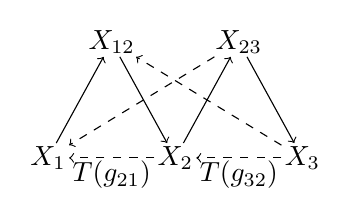
\begin{tikzpicture}[scale=0.95, every node/.style={inner sep=1pt}]
\node (X12) at (0.85,1.55) {$X_{12}$};
\node (X23) at (2.55,1.55) {$X_{23}$};
\node (X1) at (0,0) {$X_1$};
\node (X2) at (1.70,0) {$X_2$};
\node (X3) at (3.40,0) {$X_3$};
\draw[->] (X1) -- (X12);
\draw[->] (X12) -- (X2);
\draw[->] (X2) -- (X23);
\draw[->] (X23) -- (X3);
\draw[->,dashed] (X3) -- (X12);
\draw[->,dashed] (X23) -- (X1);
\draw[->,dashed] (X2) -- node[below] {$T(g_{21})$} (X1);
\draw[->,dashed] (X3) -- node[below] {$T(g_{32})$} (X2);
\end{tikzpicture}
\]

% [Tutor Note: 正誤表（2014-05-20 版）p.98 条：底本印作 $T(g_{32})\circ g_{21}=0$，应订正为 $T(g_{21})\circ g_{32}=0$。这是因为 $g_{21}\colon T^{-1}(X_2)\to X_1$、$g_{32}\colon T^{-1}(X_3)\to X_2$ 的合成 $g_{21}\circ g_{32}$ 才落在 $T^{-1}(X_2)$ 上，平移一次得 $T(g_{21})\circ g_{32}\colon T^{-1}(X_3)\to T(X_1)$，可与 $T(g_{21})$ 所在的三角序列的零复合相容。本译本正文按订正后翻译。]

$(\mathrm{Tr}5)^+$：固定 $\tilde g_{32}$ 时，可适当选取 $\tilde g_{21}$ 使交换图表 (5.5) 得以构成。

$(\mathrm{Tr}5)^-$：固定 $\tilde g_{21}$ 时，可适当选取 $\tilde g_{32}$ 使交换图表 (5.5) 得以构成。

\begin{equation}
\begin{tikzcd}[row sep=2.3em, column sep=2.4em]
{} & X_1 \arrow[r,equal] \arrow[d] & X_1 \arrow[d] & {} \\
T^{-1}X_3 \arrow[r] \arrow[d,equal] & X_{12} \arrow[r] \arrow[d] & X_{123} \arrow[r] \arrow[d] & X_3 \arrow[d,equal] \\
T^{-1}X_3 \arrow[r,"g_{32}"'] & X_2 \arrow[r] \arrow[d,"T(g_{21})"'] & X_{23} \arrow[r] \arrow[d] & X_3 \arrow[d] \\
{} & TX_1 \arrow[r,equal] & TX_1 \arrow[r] & TX_{12}
\end{tikzcd} \tag{5.5}
\end{equation}

% [Tutor Note: 底本 p.98 图式 (5.5) 依作者正誤表（E10，PDF p.224 第 3 条）须补上交换方块 $X_{23}\to X_3$、$X_3\to TX_{12}$、$TX_1\to TX_{12}$、$X_{23}\to TX_1$，其中 $X_3\to TX_{12}$ 与 $TX_1\to TX_{12}$ 分别是 (5.4) 左上的射 $T^{-1}X_3\to X_{12}$ 与 $X_1\to X_{12}$ 经 $T$ 平移所得。本译本已按订正补全（图中最右下方的方块与 $TX_{12}$）。底本原图只到 $TX_1=TX_1$ 为止。]
% [Tutor Note: (5.5) 中 $X_{123}$ 与正誤表 (6) 里的 $X_{123}$、$X'_{123}$ 的构成，是 5.2 节 p.104–105 讨论 (Tr5) 时直接算出的：$X_{123}^{i}=X_1^{i}\oplus X_2^{i}\oplus X_3^{i}$，微分矩阵的下三角块由 $d_{21},d_{32}$ 给出、上三角块 $d_{31}$ 只须满足 $d^2=0$。]

% [原文 p.99]
实际上 $(\mathrm{Tr}5)^+$、$(\mathrm{Tr}5)^-$ 都与 (Tr5) 等价。$(\mathrm{Tr}5)^+$、$(\mathrm{Tr}5)^-$ 分别就是在交换图表 (5.3)、(5.4) 中所讨论的内容本身，而交换图表 (5.5) 只是把那些交换图表的对象与态射的记号改写了一下而已。

交换图表 (5.5) 从 $(\mathrm{Tr}5)^+$、$(\mathrm{Tr}5)^-$ 的观点来看，写成下面这样更便于把握。
\[
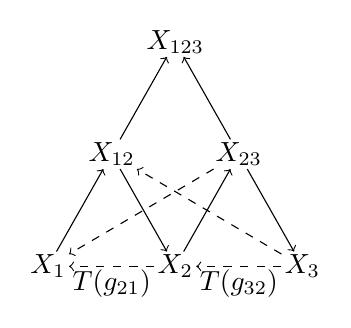
\begin{tikzpicture}[scale=0.95, every node/.style={inner sep=1pt}]
\node (X123) at (1.70,3.00) {$X_{123}$};
\node (X12) at (0.85,1.50) {$X_{12}$};
\node (X23) at (2.55,1.50) {$X_{23}$};
\node (X1) at (0,0) {$X_1$};
\node (X2) at (1.70,0) {$X_2$};
\node (X3) at (3.40,0) {$X_3$};
\draw[->] (X12) -- (X123);
\draw[->] (X23) -- (X123);
\draw[->] (X1) -- (X12);
\draw[->] (X12) -- (X2);
\draw[->] (X2) -- (X23);
\draw[->] (X23) -- (X3);
\draw[->,dashed] (X3) -- (X12);
\draw[->,dashed] (X23) -- (X1);
\draw[->,dashed] (X2) -- node[below] {$T(g_{21})$} (X1);
\draw[->,dashed] (X3) -- node[below] {$T(g_{32})$} (X2);
\end{tikzpicture}
\]

八面体公理的改写 $(\mathrm{Tr}5)^+$、$(\mathrm{Tr}5)^-$ 将在 5.2 节中从复形的写像锥的立场加以讨论。

\subsection{三角部分范畴与三角范畴的生成系}

\begin{definition}{5.17}
三角范畴 $\cT$ 的全子范畴 $\cT'$，若对 $\cT$ 的平移函子 $T$ 封闭（$T(\cT')=\cT'$），并具有由 $\cT$ 的三角结构诱导出的三角结构（即对 $\cT$ 的三角结构封闭），则称 $\cT'$ 为 $\cT$ 的全三角部分范畴（full triangulated subcategory）。
\end{definition}

说得更不含糊一些，就是：对任意对象 $X,Y\in\cT'$ 与态射 $f\colon X\to Y$，由 $\cT$ 中的正合三角序列
\[
X\xrightarrow{\,f\,} Y\to Z\to T(X)
\]
（除同构外）唯一确定的对象 $Z\in\cT$ 都是 $\cT'\subset\cT$ 的对象。

\begin{remark}{5.18}
$\cT'$ 是加法范畴。事实上，在前节的例 5.16 中，当 $u\colon X\to Y$ 是零态射时 $C(u)\simeq Y\oplus T(X)$；当 $u\colon X\to X$ 是恒等态射 $\id_X$ 时，$C(u)$ 是零对象。$\cT'$ 进一步构成三角范畴一事由定义显然可知。
\end{remark}

\begin{definition}{5.19}
给定三角范畴 $\cT$ 及其全子范畴 $\cC$。对对象 $X\in\cT$，若存在整数 $n>0$ 以及对各 $i=0,\dots,n-1$ 的 $\cT$ 的正合三角序列
\[
X_i\longrightarrow X_{i+1}\longrightarrow C_i\longrightarrow TX_i \qquad (X_0=0,\ X_n=X)
\]
使得 $C_i$ 是 $\cC$ 的对象在 $\cT$ 中的次数平移（$\exists r\in\Z$ s.t.\ $T^{-r}(C_i)\in\cC$），则称 $X$ 在 $\cT$ 中由 $\cC$ 生成（generated）。
\end{definition}

% [Tutor Note: 正誤表（2014-05-20 版）p.99 条：定义 5.19 的公式右侧须补上条件「$X_0=0$，$X_n=X$」。本译本按订正后内容把该条件写在式末括号内。另同页底本印作「与えれているとする」（应为「与えられているとする」），本译本径直译作「给定」。]

将由 $\cC$ 生成的所有对象所构成的全三角部分范畴记为 $\langle\cC\rangle$，并称其为包含 $\cC$ 的 $\cT$ 的最小全三角部分范畴。特别地，当存在三角范畴等价 $\cT\simeq\langle\cC\rangle$ 时，称 $\cC$ 为三角范畴 $\cT$ 的生成系（generator system）。

% [原文 p.100]
\begin{remark}{5.20}
上面 $X$ 由 $\cC$ 生成的条件可图示如下。
\begin{equation}
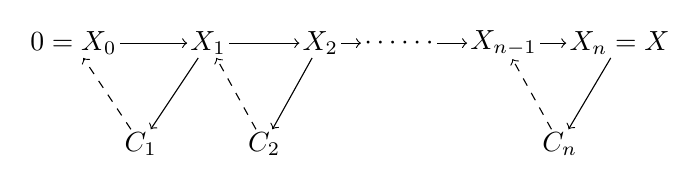
\begin{tikzpicture}[scale=0.95, every node/.style={inner sep=1pt}]
\node (X0) at (0,0) {$0=X_0$};
\node (X1) at (1.80,0) {$X_1$};
\node (X2) at (3.30,0) {$X_2$};
\node (D)  at (4.35,0) {$\cdots\cdots$};
\node (Xn1) at (5.75,0) {$X_{n-1}$};
\node (Xn) at (7.30,0) {$X_n=X$};
\node (C1) at (0.90,-1.35) {$C_1$};
\node (C2) at (2.55,-1.35) {$C_2$};
\node (Cn) at (6.50,-1.35) {$C_n$};
\draw[->] (X0) -- (X1);
\draw[->] (X1) -- (X2);
\draw[->] (X2) -- (D);
\draw[->] (D) -- (Xn1);
\draw[->] (Xn1) -- (Xn);
\draw[->,dashed] (C1) -- (X0);
\draw[->] (X1) -- (C1);
\draw[->,dashed] (C2) -- (X1);
\draw[->] (X2) -- (C2);
\draw[->,dashed] (Cn) -- (Xn1);
\draw[->] (Xn) -- (Cn);
\end{tikzpicture} \tag{5.6}
\end{equation}
其中 $X_1\simeq C_1$，$X_2$ 是态射 $T^{-1}(C_2)\to C_1$ 的写像锥，而 $X$ 是反复取这样的写像锥所得的对象。
\end{remark}

% [Tutor Note: 图 (5.6) 中虚线箭头表示次数 $+1$ 的态射：$C_i\to T(X_{i-1})$（画成指向 $X_{i-1}$ 的虚线箭头，与注意 5.2 的第二种画法一致），实线箭头则是 $X_i\to C_i$；合起来每个 $C_i$ 处是一个正合三角序列 $X_{i-1}\to X_i\to C_i\to T(X_{i-1})$。可验证锚点：$n=2$ 时该图就是 $0=X_0\to X_1\to X_2=X$，$C_1=X_1$，$C_2$ 的写像锥给出 $X$，与定义 5.19 的要求逐条对应。]

在这个定义中，取写像锥的次序看上去似乎被固定了；但由前节所讨论的八面体公理 $(\mathrm{Tr}5)^+$、$(\mathrm{Tr}5)^-$ 可知，$X$ 并不依赖于取写像锥的次序。例如 $n=3$ 时，$X=X_3$ 是
\[
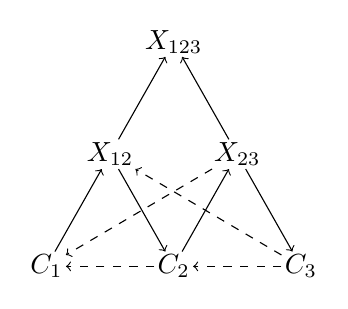
\begin{tikzpicture}[scale=0.95, every node/.style={inner sep=1pt}]
\node (X123) at (1.70,3.00) {$X_{123}$};
\node (X12) at (0.85,1.50) {$X_{12}$};
\node (X23) at (2.55,1.50) {$X_{23}$};
\node (C1) at (0,0) {$C_1$};
\node (C2) at (1.70,0) {$C_2$};
\node (C3) at (3.40,0) {$C_3$};
\draw[->] (X12) -- (X123);
\draw[->] (X23) -- (X123);
\draw[->] (C1) -- (X12);
\draw[->] (X12) -- (C2);
\draw[->] (C2) -- (X23);
\draw[->] (X23) -- (C3);
\draw[->,dashed] (C3) -- (X12);
\draw[->,dashed] (X23) -- (C1);
\draw[->,dashed] (C2) -- (C1);
\draw[->,dashed] (C3) -- (C2);
\end{tikzpicture}
\]
中取 $X_1=C_1$、$X_2=X_{12}$，并把态射 $C_3\to T(C_2)$、$C_2\to T(C_1)$ 分别取为 (5.6) 中态射的合成 $C_3\to T(X_2)\to T(C_2)$、$C_2\to T(X_1)=T(C_1)$ 时所得的 $X_{123}$；一般的 $n$ 的情形也同样地作为如此构成的金字塔的顶点而得到 $X$。此时，
\[
T^n(C_1)\longleftarrow\cdots\longleftarrow T(C_{n-1})\longleftarrow C_n
\]
构成复形，而 (5.6) 有时被称为该复形的右 Postnikov 系（Postnikov system）。(5.6) 对应金字塔的左斜面，而作为对应其右斜面者，可定义左 Postnikov 系 [17, p257]。

\section{同伦范畴的正合三角结构}

本节证明加法范畴 $\cC$ 的同伦范畴 $K(\cC)$ 构成三角范畴。$K(\cC)$ 的对象是 $\cC$ 的复形 $X := \{X^n,d^n\}_{n\in\Z}$。不仅限于向量空间的复形或 $R$-模的复形的情形（定义 3.23），对于一般加法范畴 $\cC$ 中的复形，也可定义把次数平移 1 的运算即悬垂，而它定义了三角范畴 $K(\cC)$ 中的平移函子（定义 5.6）。

\begin{definition}{5.21}[加法范畴中复形的悬垂]
设 $\cC$ 为加法范畴。对 $\cC$ 中的复形 $X := \{X^i,d^i_X\}_{i\in\Z}$，由
\[
(X[1])^i := X^{i+1},\qquad d^i_{X[1]} := -d^{i+1}_X
\]
定义复形 $X[1] := \{(X[1])^i,d^i_{X[1]}\}_{i\in\Z}$。称 $X[1]$ 为 $X$ 的悬垂（suspension）。
\end{definition}

% [原文 p.101]
\begin{definition}{5.22}
对加法范畴 $\cC$ 的复形范畴 $\Comp(\cC)$ 中的加法自同构函子 $T\colon\Comp(\cC)\to\Comp(\cC)$，如下定义。
\begin{itemize}[leftmargin=2em, itemsep=0.2em]
\item 对 $X\in\Comp(\cC)$，$T(X) := X[1]$。同样地，对 $n\in\Z$，记 $T^n(X)=X[n]$。
\item 对 $X,Y\in\Comp(\cC)$、$\phi=\{\phi^i\}_{i\in\Z}\in\Hom_{\Comp(\cC)}(X,Y)$，$T(\phi)\colon T(X)\to T(Y)$ 由
\[
(T(\phi))^i := \phi^{i+1}\colon (T(X))^i\to(T(Y))^i
\]
定义。
\end{itemize}
由此诱导出的、定义在同伦范畴 $K(\cC)$ 上的加法自同构函子用同一记号 $T\colon K(\cC)\to K(\cC)$ 表示。
\end{definition}

定义 $K(\cC)$ 的正合三角序列。在 $R$-模的复形的情形，已经讨论过：只要给定复形的态射，就必可得到对应的复形的短正合列（命题 3.26）。按那里的记号，对复形的态射 $d_{ZX}\colon Z\to X[1]$，存在复形的短正合列
\[
0\to X\to Y\to Z\to 0,
\]
其中 $Y=\{Y^n,d^n_Y\}_{n\in\Z}$ 是由
\[
Y^n := X^n\oplus Z^n,\qquad d^n_Y := d^n_X+d^n_Z+d^n_{ZX}
\]
确定的。这样的事情在一般加法范畴中也可做到。

\begin{definition}{5.23}
对加法范畴 $\cC$ 的复形 $Z,X$，当给定复形的态射 $\phi := \{\phi^i\colon Z^i\to(X[1])^i\}_{i\in\Z}$ 时，由
\[
Y^i := X^i\oplus Z^i,\qquad d^i_Y := d^i_X+d^i_Z+\phi^i
\]
定义复形 $Y := \{Y^i,d^i_Y\}_{i\in\Z}\in\Comp(\cC)$。令 $C(\phi) := TY$，并称其为复形的态射 $\phi$ 的写像锥（mapping cone）。
\end{definition}

% [Tutor Note: 底本 p.101 定义 5.23 原印作「複体 $C(\phi):=\{C(\phi)^i,d^i_{C(\phi)}\}\in\Comp(\cC)$ を $C(\phi)^i:=X^i\oplus Z^i$，$d^i_{C(\phi)}:=d^i_X+d^i_Z+\phi^i$ で定义する。$C(\phi)$ を……写像锥という。」据作者正誤表（2014-05-20 版）p.101 条，应改为：先用同一公式定义辅助复形 $Y$，再令 $C(\phi):=TY$。本译本正文按订正后翻译。附带说明：底本 p.102 在 [Tr1] 中给 $C(\id_X)$ 写出的矩阵用的是 $Y$ 的分量（$C(\id_X)^i=X^i\oplus(X[1])^i$），与 $C(\phi):=TY$ 差一次平移；两处的不一致源于底本记号混用，读者只须注意「$Y$ 是那两条正合列中的中间项，$C(\phi)$ 是它的平移」即可。]

此时，由 $\id_{X^i}\colon X^i\to X^i\subset(X^i\oplus Z^i)=Y^i$ 确定的复形的（单）态射 $u\colon X\to Y$，以及由 $Y^i=(X^i\oplus Z^i)$ 到 $Z^i$ 的投影确定的复形的（满）态射 $v\colon Y\to Z$，可得短正合列
\begin{equation}
0\longrightarrow X\xrightarrow{u}Y\xrightarrow{v}Z\longrightarrow 0,\qquad TY=C(\phi) \tag{5.7}
\end{equation}
由此可以考察三角序列
\[
X\xrightarrow{u}Y\xrightarrow{v}Z\xrightarrow{\phi}T(X).
\]
这样的三角序列称为伴随写像锥的三角序列。

% [Tutor Note: 底本 p.101 式 (5.7) 印作「$Y:=C(\phi)$」，据作者正誤表（2014-05-20 版）p.101 (5.7) 条应作「$TY=C(\phi)$」。本译本按订正后翻译。]

\begin{proposition}{5.24}
在加法范畴 $\cC$ 的同伦范畴 $K(\cC)$ 中，与伴随写像锥的三角序列同构的三角序列的全体满足正合三角序列的公理（定义 5.4），由此 $K(\cC)$ 构成三角范畴。
\end{proposition}

% [原文 p.102]
以下在本章中证明该命题。也就是说，逐一确认与伴随写像锥的三角序列 (5.7) 同构的三角序列满足正合三角序列的公理 (Tr1)–(Tr5)。

[(Tr1)] 对复形 $X := \{X^i,d^i_X\}_{i\in\Z}$，证明写像锥 $C(\id_X)$ 是 $K(\cC)$ 的零对象，即在 $\Comp(\cC)$ 中与零对象同伦等价。将 $C(\id_X) = \{C(\id_X)^i, d^i_{C(\id_X)}\}_{i\in\Z}$ 按如下方式作矩阵表示。
\[
C(\id_X)^i = \binom{X^i}{(X[1])^i},\qquad
d^i_{C(\id_X)} = \begin{pmatrix} d^i_X & \id_{(X[1])^i} \\ 0 & d^i_{X[1]}\end{pmatrix}\colon
\binom{X^i}{(X[1])^i}\longrightarrow\binom{X^{i+1}}{(X[1])^{i+1}}.
\]
设 $\Comp(\cC)$ 中的零对象与 $C(\id_X)$ 之间的零态射为 $\iota\colon 0\to C(\id_X)$、$\pi\colon C(\id_X)\to 0$，则 $\pi\circ\iota = 0_0 = \id_0$，故只须证明 $\iota\circ\pi = 0_{C(\id_X)}$ 与 $\id_{C(\id_X)}$ 同伦。对每个 $i\in\Z$，定义 $h^i\colon C(\id_X)^i\to C(\id_X)^{i-1}$ 为
\[
h^i = \begin{pmatrix} 0 & 0 \\ \id_{X^i} & 0\end{pmatrix}\colon
\binom{X^i}{(X[1])^i}\longrightarrow\binom{X^{i-1}}{(X[1])^{i-1}},
\]
则
\[
\begin{aligned}
d^{i-1}_{C(\id_X)}\circ h^i + h^{i+1}\circ d^i_{C(\id_X)}
&= \begin{pmatrix} d^{i-1}_X & \id_{(X[1])^{i-1}} \\ 0 & d^{i-1}_{X[1]}\end{pmatrix}\begin{pmatrix} 0 & 0 \\ \id_{X^i} & 0\end{pmatrix}
+ \begin{pmatrix} 0 & 0 \\ \id_{X^{i+1}} & 0\end{pmatrix}\begin{pmatrix} d^i_X & \id_{(X[1])^i} \\ 0 & d^i_{X[1]}\end{pmatrix}\\
&= \begin{pmatrix} \id_{X^i} & 0 \\ 0 & \id_{(X[1])^i}\end{pmatrix},
\end{aligned}
\]
因此证明了 $0\overset{\mathrm{h.e.}}{\sim}\id_{C(\id_X)}$。

% [Tutor Note: 这里 $h^i$ 的左上分块为 0、左下分块为 $\id_{X^i}$，正是「把 $X^i$ 平移一格后接到 $(X[1])^{i-1}=X^i$ 上」的标准同伦；最后一矩阵的左下角之所以抵消，靠的是 $d^{i-1}_{X[1]}=-d^{i}_{X}$（悬垂定义 5.21），可作逐项验算的锚点。]

[(Tr2)] 由定义显然。

[(Tr3)] 构造如下 $K(\cC)$ 中三角序列的同构。
\begin{equation}
\begin{tikzcd}[row sep=2.4em, column sep=2.4em]
X \arrow[r,"u"] \arrow[d,"\id_X"] & Y \arrow[r,"v"] \arrow[d,"\id_Y"] & Z \arrow[r,"w"] \arrow[d,"h"] & T(X) \arrow[d,"T(\id_X)"] \\
X \arrow[r,"u"] & Y \arrow[r,"v'"] & \tilde Z \arrow[r,"w'"] & T(X)
\end{tikzcd} \tag{5.8}
\end{equation}
其中 $Y=C(T^{-1}(w))$，$\tilde Z=C(u)$。

首先证明在 $\Comp(\cC)$ 中 $Z\overset{\mathrm{h.e.}}{\sim}\tilde Z$。关于 $\tilde Z := \{\tilde Z^i, d^i_{\tilde Z}\}_{i\in\Z}$，有 $\tilde Z^i = Y^i\oplus(T(X))^i = X^i\oplus Z^i\oplus(X[1])^i$，而 $d^i_{\tilde Z}$ 作矩阵表示为
% [原文 p.103]
\begin{equation}
d^i_{\tilde Z} = \begin{pmatrix} d^i_X & d^i_{ZX} & \id_{(X[1])^i} \\ 0 & d^i_Z & 0 \\ 0 & 0 & d^i_{X[1]}\end{pmatrix}\colon
\begin{pmatrix} X^i \\ Z^i \\ (X[1])^i\end{pmatrix}\longrightarrow
\begin{pmatrix} X^{i+1} \\ Z^{i+1} \\ (X[1])^{i+1}\end{pmatrix}
\end{equation}
这里设 $(T^{-1}(w))^n =: d^n_{ZX}$。下面考虑由 $\Comp(\cC)$ 的全单射（同构态射）$\psi\colon\tilde Z\to\tilde{\tilde Z}$ 给出的与 $\tilde Z$ 同构的对象 $\tilde{\tilde Z}$。
\[
\psi^i = \begin{pmatrix} 1 & 0 & 0 \\ 0 & 1 & 0 \\ -d^i_X & -d^i_{ZX} & 1\end{pmatrix}.
\]
这里把对角成分 $\id_{X^i},\id_{Z^i},\id_{(X[1])^i}$ 简写为「1」。由此，$\tilde{\tilde Z} := \{\tilde{\tilde Z}^i, d^i_{\tilde{\tilde Z}} = \psi^i\circ d^i_{\tilde Z}\circ(\psi^i)^{-1}\}_{i\in\Z}$ 满足 $\tilde{\tilde Z}^i = \tilde Z^i$，且
\[
\begin{aligned}
d^i_{\tilde{\tilde Z}}
&= \begin{pmatrix} 1 & 0 & 0 \\ 0 & 1 & 0 \\ -d^i_X & -d^i_{ZX} & 1\end{pmatrix}
\begin{pmatrix} d^i_X & d^i_{ZX} & \id_{(X[1])^i} \\ 0 & d^i_Z & 0 \\ 0 & 0 & d^i_{X[1]}\end{pmatrix}
\begin{pmatrix} 1 & 0 & 0 \\ 0 & 1 & 0 \\ d^i_X & d^i_{ZX} & 1\end{pmatrix}\\
&= \begin{pmatrix} 0 & 0 & \id_{(X[1])^i} \\ 0 & d^i_Z & 0 \\ 0 & 0 & 0\end{pmatrix}.
\end{aligned}
\]
也就是说，得到了直和分解 $\tilde{\tilde Z} = Z\oplus C(\id_X)$。这里，在上面关于 [(Tr1)] 的讨论中已看到 $C(\id_X)\overset{\mathrm{h.e.}}{\sim}0$，故可知 $\tilde{\tilde Z}\overset{\mathrm{h.e.}}{\sim}Z$。特别地，对于与该直和分解对应的复形的单射 $\iota_Z\colon Z\to\tilde{\tilde Z}$、全射 $\pi_Z\colon\tilde{\tilde Z}\to Z$，$\psi^{-1}\circ\iota_Z\colon Z\to\tilde Z$ 与 $\pi_Z\circ\psi\colon\tilde Z\to Z$ 给出 $Z$ 与 $\tilde Z$ 之间的同伦等价态射，并使上面的图式 (5.8) 交换。也就是说，得到了 (5.8) 的三角序列的同构。

[(Tr4)] 考虑两个伴随写像锥的三角序列 $(X,Y,Z;u,v,w)$、$(X',Y',Z';u',v',w')$。这里 $Y=C(T^{-1}(w))$，$Y'=C(T^{-1}(w'))$。当给定复形的态射 $\phi_X\colon X\to X'$、$\phi_Z\colon Z\to Z'$ 并使图式
\begin{equation}
\begin{tikzcd}[row sep=2.4em, column sep=3.4em]
T^{-1}(Z) \arrow[r,"T^{-1}(w)"] \arrow[d,"T^{-1}(\phi_Z)"'] & X \arrow[d,"\phi_X"] \\
T^{-1}(\tilde Z) \arrow[r,"T^{-1}(w')"'] & \tilde X
\end{tikzcd} \tag{5.9}
\end{equation}
交换时，证明存在复形的态射 $\phi_Y\colon Y\to Y'$，并可构造以下三角序列的态射。

% [Tutor Note: 底本 p.103 的图式 (5.9) 中把第二行的对象印成 $T^{-1}(\tilde Z)$、$\tilde X$（带 tilde），而 (5.10) 的第二行又用 $X',Y',Z'$（带 prime），全页 tilde 与 prime 混用。按文意，$Y=C(T^{-1}(w))$、$Y'=C(T^{-1}(w'))$，故 (5.9) 应读作 $T^{-1}(Z')\to X'$。本译本照底本印法（tilde）翻译，特此标明。]

% [原文 p.104]
\begin{equation}
\begin{tikzcd}[row sep=2.4em, column sep=2.0em]
T^{-1}(Z) \arrow[r,"T^{-1}(w)"] \arrow[d,"T^{-1}(\phi_Z)"'] & X \arrow[r,"u"] \arrow[d,"\phi_X"] & Y \arrow[r,"v"] \arrow[d,"\phi_Y"] & Z \arrow[r,"w"] \arrow[d,"\phi_Z"] & T(X) \arrow[d,"T(\phi_X)"] \\
T^{-1}(\tilde Z) \arrow[r,"T^{-1}(w')"'] & X' \arrow[r,"u'"] & Y' \arrow[r,"v'"] & Z' \arrow[r,"w'"] & T(X)
\end{tikzcd} \tag{5.10}
\end{equation}

% [Tutor Note: 正誤表（2014-05-20 版）p103 [(Tr4)] 条與 p104 (5.10) 条：底本把 $Z\to Z'$ 的态射印作 $\Phi_Z$、把 (5.10) 的竖箭頭印作 $\Phi_x,\Phi_y,\Phi_z$，均应改为小写 $\phi_Z,\phi_X,\phi_Y,\phi_Z$（$T(\Phi_x)$ 相应为 $T(\phi_X)$）。本译本正文按订正后翻译。另：底本 (5.10) 右下角印作 $T(X)$，而本行是带 prime 的三角序列，按文意应为 $T(X')$；正誤表未收此条，照译并志此疑。]

实际上，只须对 $\phi_X := \{\phi^i_X\colon X^i\to\tilde X^i\}_{i\in\Z}$、$\phi_Z := \{\phi^i_Z\colon Z^i\to\tilde Z^i\}_{i\in\Z}$ 取
\[
\phi^i_Y := \begin{pmatrix} \phi^i_X & 0 \\ 0 & \phi^i_Z\end{pmatrix}\colon
\begin{pmatrix} X^i \\ Z^i\end{pmatrix}\longrightarrow
\begin{pmatrix} X^{i+1} \\ Z^{i+1}\end{pmatrix},
\]
则 $\phi_Y := \{\phi^i_Y\}_{i\in\Z}$ 是复形的态射，且使图式 (5.10) 交换。事实上，由图式 (5.9) 的交换性，
\[
\begin{aligned}
d^i_{\tilde Y}\circ\phi^i_Y - \phi^{i+1}_Y\circ d^i_Y
&= \begin{pmatrix} d^i_{\tilde X} & w \\ 0 & d^i_{\tilde Z}\end{pmatrix}\begin{pmatrix} \phi^i_X & 0 \\ 0 & \phi^i_Z\end{pmatrix}
- \begin{pmatrix} \phi^{i+1}_X & 0 \\ 0 & \phi^{i+1}_Z\end{pmatrix}\begin{pmatrix} d^i_X & w \\ 0 & d^i_Z\end{pmatrix}\\
&= \begin{pmatrix} 0 & w\circ\phi^i_Z - \phi^{i+1}_X\circ w \\ 0 & 0\end{pmatrix} = 0,
\end{aligned}
\]
故知 $\phi_Y$ 是复形的态射。由 $\phi_Y$ 的定义，图式 (5.10) 的交换性容易看出。也就是说，可得到关于从 $X$ 到 $\tilde Y$ 的合成态射的交换性，以及关于从 $Y$ 到 $\tilde Z$ 的合成态射的交换性这两条。

% [Tutor Note: 上式右端 $w\circ\phi^i_Z-\phi^{i+1}_X\circ w$ 之所以为 0，正是 (5.9) 的可换性：$w\colon Z^i\to X^{i+1}$（即 $T^{-1}(w)$ 平移一格）满足 $\phi^{i+1}_X\circ w = w'\circ\phi^i_Z$，而竖箭頭的定义又使 $\tilde Y$ 的微分矩阵中非对角块同为 $w$。]

[(Tr5)] 证明 $K(\cC)$ 中的八面体公理。原来的八面体公理的图式是
\[
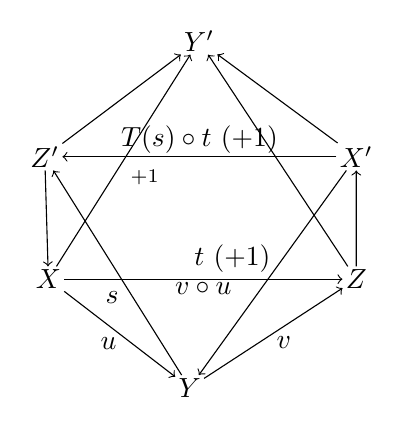
\begin{tikzpicture}[scale=0.92, every node/.style={inner sep=1pt}]
\node (Yp) at (0,2.66) {$Y'$};
\node (Zp) at (-2.13,1.06) {$Z'$};
\node (Xp) at (2.17,1.06) {$X'$};
\node (X)  at (-2.08,-0.63) {$X$};
\node (Z)  at (2.17,-0.63) {$Z$};
\node (Y)  at (-0.13,-2.13) {$Y$};
\draw[->] (Zp) -- (Yp);
\draw[->] (X)  -- (Yp);
\draw[->] (Xp) -- (Yp);
\draw[->] (Z)  -- (Yp);
\draw[->] (Xp) -- node[above] {$T(s)\circ t\ (+1)$} (Zp);
\draw[->] (Zp) -- (X);
\draw[->] (Z)  -- (Xp);
\draw[->] (X)  -- node[below] {$v\circ u$} (Z);
\draw[->] (X)  -- node[below left] {$u$} (Y);
\draw[->] (Y)  -- node[below right] {$v$} (Z);
\draw[->] (Y)  -- (Zp);
\draw[->] (Xp) -- (Y);
\node at (-1.20,-0.88) {$s$};
\node at (0.46,-0.34) {$t\ (+1)$};
\node at (-0.75,0.78) {$\scriptstyle +1$};
\end{tikzpicture}
\]
而它正是上述图式。若取 $Z'=C(u)$、$X'=C(v)$、$Y'=C(v\circ u)$ 来考虑，则
\[
(Z')^i = Y^i\oplus(X[1])^i,\qquad (X')^i = Z^i\oplus(Y[1])^i,\qquad (Y')^i = Z^i\oplus(X[1])^i,
\]
故只要把微分的结构搁在一边，就可看出「账目是相符的」。

但是这里想要确认的是八面体公理 $(\mathrm{Tr}5)^+$ 或 $(\mathrm{Tr}5)^-$ 成立。首先，关于 $g_{21}\colon T^{-1}(X_2)\to X_1$，$C(g_{21}) =: X_{12}$ 由
% [原文 p.105]
\begin{equation}
X_{12}^i = \binom{X_1^i}{X_2^i},\qquad
d^i_{X_{12}} = \begin{pmatrix} d^i_{X_1} & d^i_{21} \\ 0 & d^i_{X_2}\end{pmatrix} \tag{5.11}
\end{equation}
给出。这里设 $(T(g_{21}))^i =: d^i_{21}$。同样地，$C(g_{32}) =: X_{23}$ 由
\begin{equation}
X_{23}^i = \binom{X_2^i}{X_3^i},\qquad
d^i_{X_{23}} = \begin{pmatrix} d^i_{X_2} & d^i_{32} \\ 0 & d^i_{X_3}\end{pmatrix}, \tag{5.12}
\end{equation}
$d^i_{32} := (T(g_{32}))^i$ 给出。现在，对三角序列
\[
X_1\to X_{12}\xrightarrow{\,l\,}X_2\xrightarrow{T(g_{21})}T(X_1),\qquad
X_2\xrightarrow{\,r\,}X_{23}\to X_3\xrightarrow{T(g_{32})}T(X_2),
\]
存在满足
\begin{equation}
g_{32} = l\circ\tilde g_{32},\qquad g_{21} = \tilde g_{21}\circ T^{-1}(r) \tag{5.13}
\end{equation}
的 $\tilde g_{32}\colon T^{-1}(X_3)\to X_{12}$、$\tilde g_{21}\colon T^{-1}(X_{23})\to X_1$，而它们可作如下矩阵表示：
\[
(T(\tilde g_{32}))^i = \binom{d^i_{31}}{d^i_{32}}\colon X_3^i\longrightarrow\binom{X_1^i}{X_2^i},
\]
\[
(T(\tilde g_{21}))^i = \begin{pmatrix} d^i_{21} & (d'_{31})^i\end{pmatrix}\colon \binom{X_2^i}{X_3^i}\longrightarrow X_1^i.
\]
也就是说，由条件 (5.13)，$d^i_{21},d^i_{32}$ 就是 (5.11)、(5.12) 中的那些；而另一方面，$d_{31},d'_{31}$ 被确定为使 $\tilde g_{32},\tilde g_{21}$ 成为复形的态射。这里 $X^i_{123} = (X'_{123})^i = X_1^i\oplus X_2^i\oplus X_3^i$（作为矩阵纵向排列表示），
\[
d^i_{X_{123}} = \begin{pmatrix} d^i_{X_1} & d^i_{21} & d^i_{31} \\ 0 & d^i_{X_2} & d^i_{32} \\ 0 & 0 & d^i_{X_3}\end{pmatrix},\qquad
d^i_{X'_{123}} = \begin{pmatrix} d^i_{X_1} & d^i_{21} & (d'_{31})^i \\ 0 & d^i_{X_2} & d^i_{32} \\ 0 & 0 & d^i_{X_3}\end{pmatrix}
\]
被得到。这里，实际上使 $\tilde g_{32},\tilde g_{21}$ 成为复形的态射的关于 $d_{31},d'_{31}$ 的条件，可分别表为 $d^{i+1}_{X_{123}}\circ d^i_{X_{123}}=0$、$d^{i+1}_{X'_{123}}\circ d^i_{X'_{123}}=0$。两者形式相同，故就 $X_{123}$ 来考虑。把关于 $d_{31}$ 的条件具体写出，则为
\[
(d^{i+1}_{X_1}\circ d^i_{31} + d^{i+1}_{31}\circ d^i_{X_3}) + d^{i+1}_{21}\circ d^i_{32} = 0.
\]
由最初的假设，$d_{21}\circ d_{32}$ 在 $K(\cC)$ 中是零态射。也就是说，它在 $\Comp(\cC)$ 中与零态射同伦，故由此可知满足上述条件的 $d_{31}$ 存在。因此，若把 $\tilde g_{21},\tilde g_{32}$ 取成使 $d_{31}=d'_{31}$，则可知 $X_{123}=X'_{123}$。也就是说，八面体公理（以及与之等价的条件）得证。\hfill$\square$

% [Tutor Note: p.105 末「八面体公理（と等価な条件）が示された」で命题 5.24 の証明は終わるが、正誤表 E11 第 4 条指出：此处其实只说到「由三角序列可得 $X_{123}=X'_{123}$」，还须验证正誤表图 (6) 中四个小方块的交换性才算完整；作者说明这四个交换性在按书中方式构造 $X_{123}$ 时可直接验证（其中三个很容易，最末一个 $X_{23}\to X_3$、$TX_1\to TX_{12}$ 需多一步：两条合成在复形范畴中并不相等，只同伦），故本书省略。本译本据此加注，不改正文。]
% [Tutor Note: 可验证锚点：取 $\cC=K$-向量空间范畴、$X_1,X_2,X_3$ 为单点复形（只有一次非零项），则 $X_{12}$ 的微分块 $d_{21}$、$X_{23}$ 的 $d_{32}$ 满足 $d_{21}\circ d_{32}=0$ 是平凡条件，$d_{31}$ 可取 0，此时 $X_{123}=X'_{123}$ 立刻可见；这也说明一般情形下 $d_{31}$ 的选取正是「$d_{21}\circ d_{32}$ 同伦于零」所提供的自由度。]
